\section{Experiments}\label{sec:experiments}
We first evaluate skill retention during base-policy learning in CDPR simulation, then intermediate feedback for composition on LIBERO-Spatial, and finally complete-task CDPR adaptation. The ongoing WX200 evaluation extends the approach to another embodiment.

The CDPR simulation uses MuJoCo Warp/MJ-Lab, four object categories (apple, orange, potato, and tomato), and plate or bowl destinations. The action interface controls Cartesian translation, yaw, and the gripper.

\subsection{Base-Policy Skill Learning and Retention}\label{sec:skill_retention}
These measurements concern dense-reward training of simple CDPR skills and their consolidation into a base policy, before full-task composition. Each skill uses the instruction and reset protocol in Section~\ref{sec:skill_acquisition}; placement tests start with the object already held. Learning a new skill can degrade previously learned behavior, although the same policy must retain all component skills to execute the complete multi-stage task.

In a forgetting evaluation, mean reaching success falls from 64.1\% for the reaching reference to 5.3\% after placement RL, over three evaluation rounds per condition. The recovery evaluation in Fig.~\ref{fig:retention} is a separate measurement: balanced self-imitation raises reaching success from 8.0\% to 31.1\%. Plate placement changes from 50.0\% to 52.3\%, and bowl placement from 23.05\% to 27.65\%. The bank combines earlier reaching successes with current placement successes, balancing the retained data by instruction.

\begin{figure*}[!t]
\centering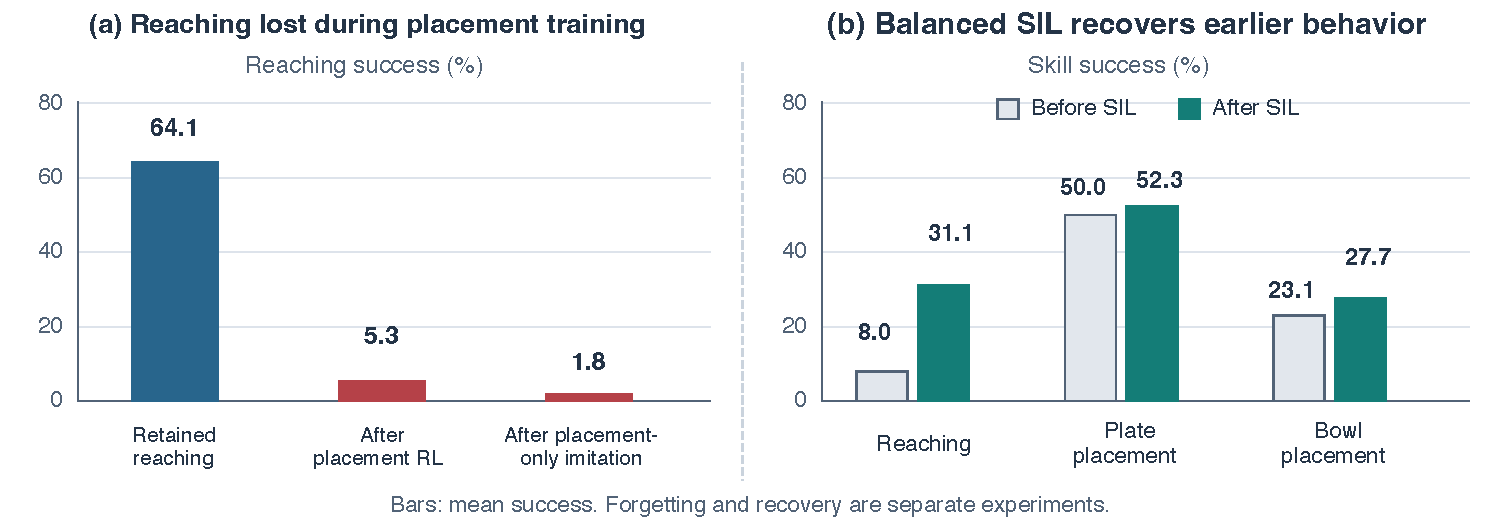
\includegraphics[width=\textwidth]{figures/skill_retention.pdf}
\caption{Base-policy skill recovery before full-task composition. Bars show means across three evaluation rounds for reaching and two rounds for each placement skill, per condition. Reaching uses the instruction \emph{move to \textless object\textgreater}; placement starts with the object already held. Reaching partially recovers while both placement means increase.}
\label{fig:retention}
\end{figure*}

Recovery is partial, with placement performance retained while reaching improves. These measurements cover approach and placement and do not isolate the contribution of self-imitation to final full-task success.


\subsection{Intermediate Feedback for Full-Task Composition}\label{sec:libero_results}
We fine-tune an OpenVLA-OFT-based policy with SimpleVLA-RL and LoRA on complete instructions for the ten LIBERO-Spatial tasks~\cite{openvlaoft,simplevlarl,libero}, using the feedback variants in Section~\ref{sec:composition}. All runs share a 61.0\% initialization and use 300 validation rollouts per endpoint. The dense-and-phase and terminal-only conditions use terminal verifier coefficient 5 and a 160-update budget. The phase-only condition uses phase-completion bonuses with terminal verifier coefficient 1 and a 110-update budget.

Dense-and-phase feedback reaches 65.3\% success versus 61.7\% for terminal-only SimpleVLA-RL (Table~\ref{tab:libero}). Phase-only feedback reaches 62.3\%, improving on the 61.0\% initialization using completion events as intermediate feedback.

For the adaptation pipeline, we use dense rewards to acquire the initial base policy on simple skills, then train the complete multi-stage task with staged reward. Milestone completion supplies intermediate credit without requiring a continuous progress function for every phase of each new instruction.
\begin{table}[!ht]
\caption{LIBERO-Spatial reward comparison from a 61.0\% initialization. Success is reported in percent; $\Delta$ is the gain in percentage points.}
\label{tab:libero}\centering\small
\begin{tabular}{@{}lrrr@{}}\toprule
Configuration & Updates & Success & $\Delta$\\\midrule
Terminal only (SimpleVLA-RL~\cite{simplevlarl}) & 160 & 61.7 & +0.7\\
Dense + phase & 160 & 65.3 & +4.3\\
Phase-only & 110 & 62.3 & +1.3\\
\bottomrule
\end{tabular}
\end{table}



\subsection{SmolVLA: Complete-Task Adaptation}\label{sec:cdpr_results}
Strict success requires grasp, held lift, intentional release, and correct placement, without carry slip or wrong-placement events.

The development validation comprises 1,024 full-task episodes: 512 plate and 512 bowl attempts. Each attempt starts with an empty gripper and uses one full-task instruction, without teacher assistance. All attempts, including numerical failures, remain in the denominator.
The adapted controller completes 723 of 1,024 development validation attempts (70.61\% strict success; Table~\ref{tab:cdpr}). Physical grasp occurs in 92.48\% of attempts and held lift in 88.28\%. Completion rates are 393/512 (76.76\%) for plates and 330/512 (64.45\%) for bowls. Carry slips (16.70\%) and wrong placements (14.16\%) remain the main failure modes.
\begin{table}[!ht]
\caption{CDPR complete task development evaluation.}
\label{tab:cdpr}\centering\small
\begin{tabular}{@{}lr@{}}\toprule
Outcome & Attempts (\%)\\\midrule
Physical grasp & 92.48\\
Held lift & 88.28\\
Strict completion (723/1,024) & 70.61\\
Carry slip & 16.70\\
Wrong placement & 14.16\\\bottomrule
\end{tabular}
\end{table}



\subsection{Additional Embodiment: WX200}\label{sec:wx200}
An ongoing experiment applies the pipeline to the five-DoF WX200 serial manipulator. This setting changes the robot mechanism while retaining the skill-learning and composition schedule. Figure~\ref{fig:wx200} reserves the setup and rollout illustrations. Quantitative success rates will be added after the evaluation is complete.

\begin{figure*}[!t]
\centering
\IfFileExists{figures/wx200/panel.pdf}{\includegraphics[width=\textwidth]{figures/wx200/panel.pdf}}{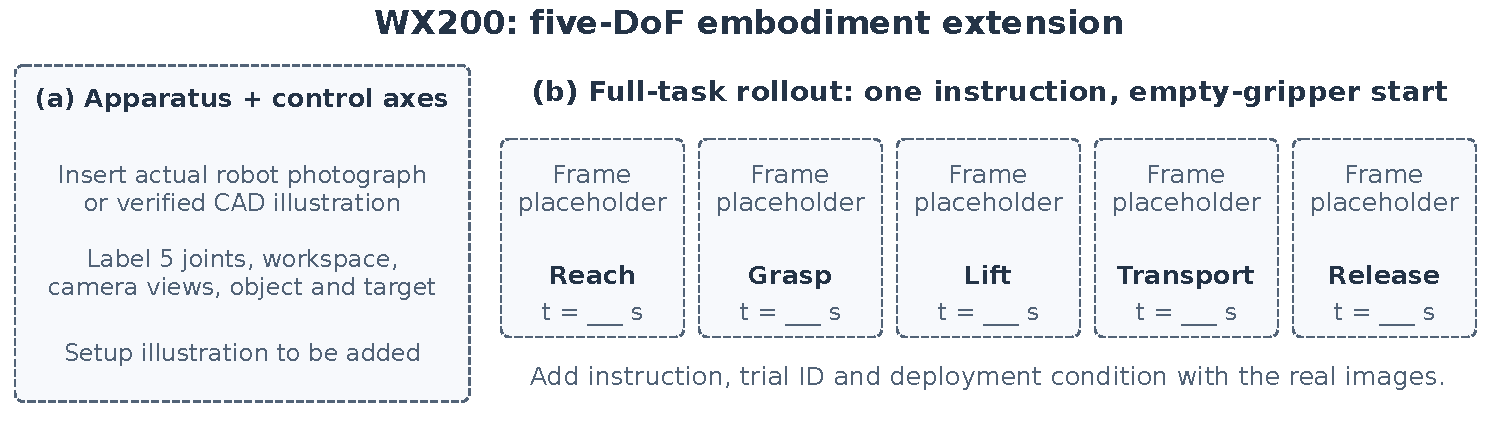
\includegraphics[width=\textwidth]{figures/wx200_slots.pdf}}
\caption{WX200 evaluation layout. (a) Apparatus, workspace, cameras, and control axes. (b) Reach, grasp, lift, transport, and release under one instruction. The current panels reserve space for setup images and timestamped rollout frames from the ongoing experiment.}
\label{fig:wx200}
\end{figure*}

\subsection{Scope of the Evidence}
The LIBERO comparisons evaluate reward variants on complete manipulation instructions. In the adaptation pipeline, dense rewards are used only for initial simple-skill acquisition; the CDPR full-task controller is trained with binary milestone feedback. The complete-task result comes from one SmolVLA training lineage and a development validation panel used during training. Retention measurements cover a small number of rounds. Earlier assisted training is part of the inherited CDPR policy; the reported full-task evaluation uses no assistance.

